%%%%%%%%%%%%%%%%%%%%%%%%%%%%%%%%%%%%%%%%%%%%%%%%%%%%%%
\documentclass[11pt]{article}
%%%%%%%%%%%%%%%%%%%%%%%%%%%%%%%%%%%%%%%%%%%%%%%%%%%%%%

\usepackage{amsmath}
\usepackage{amsthm}
\usepackage{amssymb}
\usepackage{latexsym}
\usepackage{graphicx}
\usepackage{color}
\usepackage{verbatim}
\usepackage{float}
\usepackage{multicol}
\usepackage{xcolor}
\usepackage{listings}
\usepackage{tikz}
\usetikzlibrary{arrows.meta, positioning, calc}
\usetikzlibrary{decorations.pathmorphing}
\usepackage{tcolorbox}
\tcbuselibrary{breakable}
\usepackage{cancel}


\newtcolorbox{solutionbox}{
  breakable,
  colback=blue!5!white,
  colframe=blue!50!black,
  title=Solution,
  sharp corners,
  boxrule=0.8pt
}

\newtcolorbox{hintbox}{
  breakable,
  colback=gray!10!white,
  colframe=gray!50!black,
  title=Hint,
  sharp corners,
  boxrule=0.5pt
}

% Unnumbered theorem
\newtheorem*{thm*}{Theorem}

\lstdefinelanguage{R}{
      keywords={if,else,while,for,in,next,break,function,TRUE,FALSE,NULL,Inf,NA,NaN,switch,repeat,return,require,library},
      keywordstyle=\color{blue}\bfseries,
      identifierstyle=\color{black},
      comment=[l]{\#},
      commentstyle=\color{gray}\ttfamily,
      string=[b]{"},
      stringstyle=\color{red}\ttfamily,
      morecomment=[l]{//},
      morestring=[b]{'},
      sensitive=true,
      morekeywords={print,summary,plot,lm,glm,data,frame,read.csv,write.csv,factor,levels,names,colnames,rownames,
      head,tail,str,dim,length,class,typeof,mode,is.na,is.null,is.finite,is.infinite,is.nan,as.numeric,as.character,
      as.factor,as.Date,as.POSIXct,as.matrix,as.data.frame,rbind,cbind,merge,subset,aggregate,tapply,apply,lapply,sapply,
      mapply,vapply,replicate,seq,rep,c,list,matrix,array,data.frame,table,hist,boxplot,barplot,pie,curve,lines,points,text,
      abline,legend,par,mtext,title,xlab,ylab,xlim,ylim,main,sub,col,pch,cex,lty,lwd,type,bg,fg,args,options,warnings,errors,
      message,stop,warning,error,try,tryCatch,withCallingHandlers,on.exit,debug,browser,trace,recover,options,getOption,setOption},
    }


\setlength{\textheight}{9in}
\setlength{\textwidth}{6in}
\addtolength{\topmargin}{-2cm}
\addtolength{\oddsidemargin}{-1cm}
\parindent=0in


\def\classnum{3810}
\def\classtitle{Probability}
\def\classtitleshort{Probability}
\def\classsec{001}
\def\classterm{Fall 2025}
\def\instructor{Robert Rostermundt}
%\def\hmwknum{\#2}


%%%%%%%%%%%%%%%%%%%%%%%%%%%%%%%%%%%%%%%%%%%%%%%%%%%%%%%%%
%%%%%%%%%%%%%%%%%%%%%%%%%  Colors  %%%%%%%%%%%%%%%%%%%%%%
%%%%%%%%%%%%%%%%%%%%%%%%%%%%%%%%%%%%%%%%%%%%%%%%%%%%%%%%%

\definecolor{Green}{rgb}{0,.5,0}
%use for definitions
\definecolor{Red}{rgb}{.8,.2,0}
%use for emphasis
\definecolor{Yellow}{rgb}{.6,.6,.1}
%use for part titles
\definecolor{Cyan}{rgb}{.2,.6,.7}
%use for comments
\definecolor{Purple}{rgb}{.4,0,1}
%use for examples
\definecolor{deepred}{rgb}{.53,.29,.24}
%use for important points
\definecolor{Black}{rgb}{0,0,0}
%use for washout
\definecolor{Grey}{rgb}{.45,.45,.45}
% use for theorems
\newcommand{\tred}[1]{\textcolor{Red}{#1}}
\newcommand{\tgreen}[1]{\textcolor{Green}{#1}}
\newcommand{\tcyan}[1]{\textcolor{Cyan}{#1}}
\newcommand{\tyellow}[1]{\textcolor{Yellow}{#1}}
\newcommand{\tpurple}[1]{\textcolor{Purple}{#1}}
\newcommand{\tblack}[1]{\textcolor{Black}{#1}}
\newcommand{\tgrey}[1]{\textcolor{Grey}{#1}}
\newcommand{\tdeepred}[1]{\textcolor{deepred}{#1}}
\newcommand{\ttt}[1]{\texttt{#1}}

%%%%%%%%%%%%%%%%%%%%%%%%%%%%%%%%%%%%%%%%%%%%%%%%%%%%%%%%%
%%%%%%%%%%%%%%%%%%%%%%%%%  Theorem Environments  %%%%%%%%
%%%%%%%%%%%%%%%%%%%%%%%%%%%%%%%%%%%%%%%%%%%%%%%%%%%%%%%%%

\theoremstyle{plain}
\newtheorem{thm}{Theorem}
\newtheorem{axiom}{Axiom}
\newtheorem{cor}{Corollary}
\newtheorem{lemma}{Lemma}
\newtheorem{prop}{Proposition}
\newtheorem{ques}{Question}
\theoremstyle{definition}
\newtheorem{defn}{Definition}
\theoremstyle{remark}
\newtheorem{remark}{Remark}
\theoremstyle{definition}
\newtheorem{ex}{Example}
\numberwithin{equation}{section}
\newtheorem{prob}{Problem}
\numberwithin{equation}{section}


%%%%%%%%%%%%%%%%%%%%%%%%%%%%%%%%%%%%%%%%%%%%%%%%%%%%%%%%%
%%%%%%%%%%%%%%%%%%%%%%%%%  Math    %%%%%%%%%%%%%%%%%%%%%%
%%%%%%%%%%%%%%%%%%%%%%%%%%%%%%%%%%%%%%%%%%%%%%%%%%%%%%%%%


\newcommand{\abs}[1]{\left\lvert{#1}\right\rvert}
\newcommand{\card}[1]{\lvert{#1}\rvert}
\newcommand{\union}{\cup}
\newcommand{\Union}{\bigcup}
\newcommand{\inter}{\cap}
\newcommand{\Inter}{\bigcap}
%\newcommand{\hint}[1]{\medskip\newline\emph{Hint: #1}}
%\newcommand{\note}[1]{\medskip\newline\emph{Note: #1}}
\newcommand{\points}[1]{[#1 points]}
\newcommand{\totalpoints}[1]{[#1 points total]}
\newcommand{\ds}{\displaystyle}
\newcommand{\ben}{\begin{enumerate}}
\newcommand{\een}{\end{enumerate}}
\newcommand{\bi}{\begin{itemize}}
\newcommand{\ei}{\end{itemize}}
\newcommand{\beq}{\begin{eqnarray*}}
\newcommand{\eeq}{\end{eqnarray*}}
\newcommand{\bieq}{\begin{IEEEeqnarray}{rCl}}
\newcommand{\bieqx}{\begin{IEEEeqnarray}{+rCl+x*}}
\newcommand{\eieq}{\end{IEEEeqnarray}}
\newcommand{\nn}{\nonumber}
%\renewcommand{\i}{\item}
\newcommand{\bpm}{\begin{pmatrix}}
\newcommand{\epm}{\end{pmatrix}}
\newcommand{\sol}{\indent{\bf\emph{Solution:}}}
\newcommand{\ssol}{\indent{\\[2mm]\bf\emph{Solution:}}\;}
\newcommand{\hint}{\indent{\bf\emph{Hint}:}\;}
\newcommand{\note}{\indent{\bf\emph{Note}:}\;}
\newcommand{\vsk}{\vskip 2mm}
%%%%%%%%%%%%%%%%%%%%%%%%% Calculus %%%%%%%%%%%%%%%%%%%%%%%%%%%%
\newcommand{\dd}[2]{\ds\frac{d}{d{#1}}\left[{#2}\right]}
\newcommand{\der}[2]{\ds\frac{d{#1}}{d{#2}}}
\newcommand{\lmt}[3]{\ds\lim_{{#1}\to{#2}}{#3}}
\renewcommand{\iint}[2]{\ds\int{#1}\,d{#2}}
\newcommand{\dint}[4]{\ds\int^{#4}_{#3}{#1}\,d{#2}}
\renewcommand{\Delta}{\triangle}
%%%%%%%%%%%%%%%%%%%%%%%%% Number Sets %%%%%%%%%%%%%%%%%%%%%%%%%%
\newcommand{\N}{\mathbb{N}}
\newcommand{\Z}{\mathbb{Z}}
\newcommand{\Q}{\mathbb{Q}}
\newcommand{\R}{\mathbb{R}}
\newcommand{\C}{\mathbb{C}}
\newcommand{\F}{\mathcal{F}}
\renewcommand{\P}{\mathbb{P}}
\newcommand{\E}{\mathcal{E}}
\renewcommand{\o}{\omega}
\renewcommand{\O}{\Omega}
%%%%%%%%%%%%%%%%%%%%%%%%% Vectors %%%%%%%%%%%%%%%%%%%%%%%%%%%%%
\newcommand{\x}{\bar{x}}
\renewcommand{\v}{\bar{v}}
\newcommand{\y}{\bar{y}}
\newcommand{\z}{\bar{z}}
\newcommand{\w}{\bar{w}}
\renewcommand{\u}{\bar{u}}
\renewcommand{\b}{\bar{b}}
\newcommand{\e}{\bar{e}}
\renewcommand{\a}{\vec{a}}
\renewcommand{\r}{\vec{r}}
\newcommand{\vv}{\vec{v}}
\newcommand{\vecPQ}[2]{\overrightarrow{#1}{#2}}
\newcommand{\vecV}[1]{\overrightarrow{#1}}
\newcommand{\la}{\langle}
\newcommand{\ra}{\rangle}
%%%%%%%%%%%%%%%%%%%%%%%%%%% Vector Spaces %%%%%%%%%%%%%%%%%%%%
\newcommand{\rn}{\ensuremath{\mathbb{R}^n}}
\renewcommand{\rm}{\ensuremath{\mathbb{R}^m}}
\newcommand{\re}{\mathbb{R}}
\newcommand{\Pn}{\mathbb{P}_n}
\newcommand{\B}{\mathcal{B}}
%%%%%%%%%%%%%%%%%%%%%%%%%%% Graphics %%%%%%%%%%%%%%%%%%%%%%%%
\newcommand{\cg}[2]{\begin{center}
\includegraphics[scale={#1}]{{#2}}
\end{center}}
\makeatletter
\def\imod#1{\allowbreak\mkern10mu({\operator@font mod}\,\,#1)}
\makeatother

%%%%%%%%%%%%%%%%%%%%%%%%%%%%%%%%%%%%%%%%%%%%%%%%%%%%%%%%%%%%%%%%%%%%%%%%%%%%%%%%%%%%%%%%%%%%%%
%%%%%%%%%%%%%%%%%%%%%%%%%%%%%% Defined Fonts %%%%%%%%%%%%%%%%%%%%%%%%%%%%%%%%%%%%%%%%%%%%%%%%%
%%%%%%%%%%%%%%%%%%%%%%%%%%%%%%%%%%%%%%%%%%%%%%%%%%%%%%%%%%%%%%%%%%%%%%%%%%%%%%%%%%%%%%%%%%%%%%

\font\minihelv=phvr at 6pt
\font\helv=phvr at 10pt
\font\medhelv=phvr at 16pt
\font\bighelv=phvr at 20pt
\font\hugehelv=phvr at 36pt
\font\mybigfont=phvr at 16pt
\font\mymediumfont=phvr at 14pt
\font\mediumhelv=phvr at 14pt
\font\mybfit=ptmbi at 12pt


%%%%%%%%%%%%%%%%%%%%%%%%%%%%%%%%%%%%%%%%%%%%%%%%%%%%%%%%%%%%%%%%%%%%%%%%%%%%%%%%%%%%%%%%%%%%%%%
%%%%%%%%%%%%%%%%%%%%%%%%%%%%%% Other Commands %%%%%%%%%%%%%%%%%%%%%%%%%%%%%%%%%%%%%%%%%%%%%%%%%
%%%%%%%%%%%%%%%%%%%%%%%%%%%%%%%%%%%%%%%%%%%%%%%%%%%%%%%%%%%%%%%%%%%%%%%%%%%%%%%%%%%%%%%%%%%%%%%
%\setlength\fboxrule{.5pt}
%\newcommand{\latexpicborder}[3]{
%\setlength\fboxsep{30pt}
%\begin{figure}[hb]
%\begin{center}
%\fbox{
%\input{#1}
%}
%\caption{#2}
%\label{#3}
%\end{center}
%\end{figure}
%\setlength\fboxsep{0pt}
%}
%
%\newcommand{\latexpic}[2]{
%\begin{figure}[hb]
%\begin{center}
%\input{#1}
%\vspace*{8mm}
%\caption{#2}
%\end{center}
%\end{figure}
%}

%\begin{minipage}[b]{0.6\linewidth}
%......
%\end{minipage}
%\hspace{0.5cm}
%\begin{minipage}[t]{0.4\linewidth}
%\centering
%\includegraphics[scale=.5]{m1401_ex3_g4.eps}
%\end{minipage}
%\end{figure}


%%%%%%%%%%%%%%%%%%%%%%%%%%%%%%%%%%%%%%%%%%%%%%%%%%%%%%%%%%%%%%%%%%%%%%%%%%%%%%%%%%%%%%%%%%%%%%
%%%%%%%%%%%%%%%%%%%%%%%%%%% IEEEeqnarray Notes %%%%%%%%%%%%%%%%%%%%%%%%%%%%%%%%%%%%%%%%%%%%%%%
%%%%%%%%%%%%%%%%%%%%%%%%%%%%%%%%%%%%%%%%%%%%%%%%%%%%%%%%%%%%%%%%%%%%%%%%%%%%%%%%%%%%%%%%%%%%%%


%Any number of columns can be specified with IEEEeqnarray: {c} will give only one
%column with all entries centered, or {rCll} would add a fourth, left-justified
%column to use for comments. Moreover, beside l, c, r, L, C, R for math mode
%entries there are also s, t, u for left, centered, and right text mode entries.
%Additional space can be added with . and / and ? in increasing order.
%
%
%\begin{proof}
%This is a proof that ends
%with an equation array:
%\begin{IEEEeqnarray*}{+rCl+x*}
%a & = & b + c \\
%& = & d + e. & \qedhere
%\end{IEEEeqnarray*}
%\end{proof}
%Note that the + in {+rCl+x*} denotes stretchable spaces, one on the left
%of the equations (which, if not specified, will be done automatically by
%IEEEeqnarray!) and one on the right of the equations. But now on the right,
%after the stretching column, we add an empty column x. This column will be
%only needed on the last line when we will put the \qedhere command there.
%Finally, we specify a *. This is a null-space that prevents IEEEeqnarray to
%add another unwanted +-space!


% The following environments enable custom numbering of theorems so that the numbers agree % with the numbering in the textbook being used. 
%
%  Usage examples:
%\begin{customthm}{2.2}\label{eight}
%Every theorem must be numbered by hand.
%\end{customthm}
%
%Here is a reference to theorem~\ref{eight}.
%
%\begin{customthm}{2.3}[Parenthetical comment]\label{nine}
%Statement
%\end{customthm}
%
%Here is a reference to theorem~\ref{nine}


\newtheorem{innercustomthm}{Theorem}
\newenvironment{customthm}[1]
  {\renewcommand\theinnercustomthm{#1}\innercustomthm}
  {\endinnercustomthm}
  
  \newtheorem{innercustomprop}{Proposition}
\newenvironment{customprop}[1]
  {\renewcommand\theinnercustomprop{#1}\innercustomprop}
  {\endinnercustomprop}
  
    \newtheorem{innercustomlem}{Lemma}
\newenvironment{customlem}[1]
  {\renewcommand\theinnercustomlem{#1}\innercustomlem}
  {\endinnercustomlem}
  
    \newtheorem{innercustomconj}{Conjecture}
\newenvironment{customconj}[1]
  {\renewcommand\theinnercustomconj{#1}\innercustomconj}
  {\endinnercustomconj}
  
    \newtheorem{innercustomclaim}{Claim}
\newenvironment{customclaim}[1]
  {\renewcommand\theinnercustomclaim{#1}\innercustomclaim}
  {\endinnercustomclaim}
  
    \newtheorem{innercustomcor}{Corollary}
\newenvironment{customcor}[1]
  {\renewcommand\theinnercustomcor{#1}\innercustomcor}
  {\endinnercustomcor}
  
    \newtheorem{innercustomdef}{Definition}
\newenvironment{customdef}[1]
  {\renewcommand\theinnercustomdef{#1}\innercustomdef}
  {\endinnercustomdef}
  
    \newtheorem{innercustomex}{Example}
\newenvironment{customex}[1]
  {\renewcommand\theinnercustomex{#1}\innercustomex}
  {\endinnercustomex}
  
    \newtheorem{innercustomass}{Assumption}
\newenvironment{customass}[1]
  {\renewcommand\theinnercustomass{#1}\innercustomass}
  {\endinnercustomass}
  
      \newtheorem{innercustomax}{Axiom}
\newenvironment{customax}[1]
  {\renewcommand\theinnercustomax{#1}\innercustomax}
  {\endinnercustomax}
  

\vfuzz2pt % Don't report over-full v-boxes if over-edge is small
\hfuzz2pt % Don't report over-full h-boxes if over-edge is small

\renewcommand{\ni}{\noindent}


%%%%%%%%%%%%%%%%%%%%%%%%%%%%%%%%%%%%%%%%%%%%%%%%%%%%%%
%%%%%%%%%%%%%%%%%%%%%%%%%%%%%%%%%%%%%%%%%%%%%%%%%%%%%%

\pagestyle{myheadings}

%%%%%%%%%%%%%%%%%%%%%%%%%%%%%%%%%%%%%%%%%%%%%%%%%%%%%%

%%%%%%%%%%%%%%%%%%%%%%%%%%%%%%%%%%%%%%%%%%%%%%%%%%%%%%
%%%%%%%%%%%%%%%%%%%%%%%%%   Document Body   %%%%%%%%%%
%%%%%%%%%%%%%%%%%%%%%%%%%%%%%%%%%%%%%%%%%%%%%%%%%%%%%%

%\def\classnum{3810}
%\def\classtitle{Probability}
%\def\classtitleshort{Probability}
%\def\classsec{001}
%\def\classterm{Fall 2025}
%\def\instructor{Robert Rostermundt}
\def\printsol{0}


	\title{\vspace{-1in}Math\classnum\;-\;\classtitle\\
	Section\;\classsec\;-\;\classterm\\
	Notes: Continuous Random Variables}
	\author{University of Colorado Denver / College of Liberal Arts 	and Sciences}
	\date{Department of Mathematics - \instructor}

	\markright{Math\classnum\;-\;\classtitleshort, UCD, \classterm, \instructor}



%%%%%%%%%%%%%%%%%%%%%%%%%%%%%%%%%%%%%%%%%%%%%%%%%%%%%%
\begin{document}\maketitle\thispagestyle{empty}
%%%%%%%%%%%%%%%%%%%%%%%%%%%%%%%%%%%%%%%%%%%%%%%%%%%%%%



%%%%%%%%%%%%%%%%%%%%%%%%%%%%%%%%%%%%%%%%%%%%%%%%%%%%%%%%%%%%%%%%%%%%%%%%%%%%%%%%%%%%%%%%%%%%%%%%%%%%%%
\vspace*{2mm}
\hrule
\vskip 8mm



%%%%%%%%%%%%%%%%%%%%%%%%%%%%%%%%%%%%%%%%%%%%%%%%%%%%%%%%%%%%%%%%%%%%%%%%%%%%%%%%%%%%%%%%%%%%%%%%%%%%%%
\section*{Motivation:}
%%%%%%%%%%%%%%%%%%%%%%%%%%%%%%%%%%%%%%%%%%%%%%%%%%%%%%%%%%%%%%%%%%%%%%%%%%%%%%%%%%%%%%%%%%%%%%%%%%%%%%


\noindent In probability theory, a \emph{random variable} is a way of assigning a numerical value to each outcome in a probability space. This allows us to quantify uncertain events and compute probabilities, expected values, and other statistical measures.

\medskip

\textbf{Motivating example: Gambling with dice.} Suppose you roll two fair six-sided dice. Let the sample space be 
\[
\Omega = \{(i,j) : i,j = 1,2,3,4,5,6\}.
\] 
Instead of only asking about which pair of numbers appears, imagine a gambling game where you receive different monetary payouts depending on the dice roll:
\begin{itemize}
    \item If the sum of the dice is 7, you win \$10.
    \item If the sum is 2 or 12, you win \$5.
    \item Otherwise, you lose \$2.
\end{itemize}

Here, the \emph{random variable} \(X\) represents your winnings: 
\[
X: \Omega \to \mathbb{R}, \quad X(i,j) =
\begin{cases} 
10 & \text{if } i+j = 7,\\
5 & \text{if } i+j = 2 \text{ or } 12,\\
-2 & \text{otherwise}.
\end{cases}
\]

This example illustrates the general idea: a random variable maps each outcome \(\omega \in \Omega\) to a numerical value \(X(\omega)\). Once we have \(X\), we can compute probabilities of events such as “winning money” (\(X>0\)), the expected payout, or other statistics of interest.  

\medskip

This perspective allows us to move beyond simple outcomes and reason about numerical quantities associated with complex events in any probability model. Let's quickly review some basic concepts about general random variables. 


%%%%%%%%%%%%%%%%%%%%%%%%%%%%%%%%%%%%%%%%%%%%%%%%%%%%%%%%%%%%%%%%%%%%%%%%%%%%%%%%%%%%%%%%%%%%%%%%%%%%%%
\section*{General Random Variables:}
%%%%%%%%%%%%%%%%%%%%%%%%%%%%%%%%%%%%%%%%%%%%%%%%%%%%%%%%%%%%%%%%%%%%%%%%%%%%%%%%%%%%%%%%%%%%%%%%%%%%%%


\begin{defn}
Given a probability space $(\O,\F,\P)$, a {\bf\emph{random variable}} is an $\F$-measurable function $X:\O\to\R$.
\end{defn}

\ni {\bf\emph{Note}}: An $\F$-measureable function is a function so that for every Borel set $B\in 2^{\R}$, we must have the preimage $X^{-1}(B)\in\F$; i.e., 
\[X^{-1}(B)=\left\{\o\in\O:X(\o)\in B\right\}\in\F.\]
If we let $\mathcal{C}_0$ be the set of all open intervals on the real line, we call the smallest $\sigma$-algebra containing 
$\mathcal{C}_0$, denoted $\mathcal{B}(\R)$, the Borel $\sigma$-algebra. A Borel set is an element of $\mathcal{B}(\R)$. The point is we need to be able to assign probabilities to the set $X^{-1}(\mathcal{B})$, and so all such preimages must be events.\\

\ni We want to assign probabilities to subsets of $Im(X)$. That is, we want to assign a {\bf\emph{probability law}}, denoted $\P_{X}$, to $X$. We do this in the following way: 
\[\P_{_X}:\mathcal{B}(\R)\to[0,1],\text{ where }\P_{_X}\big(B\big)\mapsto\P\big(X^{-1}(B)\big).\]
So the probability law for $X$ is the composition of $X^{-1}$ and the original probability measure $\P$. That is, 
\[\P_{_X}=\P\circ X^{-1}.\] 
See the diagram in Figure~\ref{fig:problaw} below.
\vskip 1cm

%%%%%%%%%%%%%%%%%%%%%%%%%%%%%%%%%%%%%%%%%%%%%%%%%%%%%%%%%%%%%%%%%%%%
% Randon Variable Diagram
%%%%%%%%%%%%%%%%%%%%%%%%%%%%%%%%%%%%%%%%%%%%%%%%%%%%%%%%%%%%%%%%%%%%

\begin{figure}[h!]
	\begin{center}
		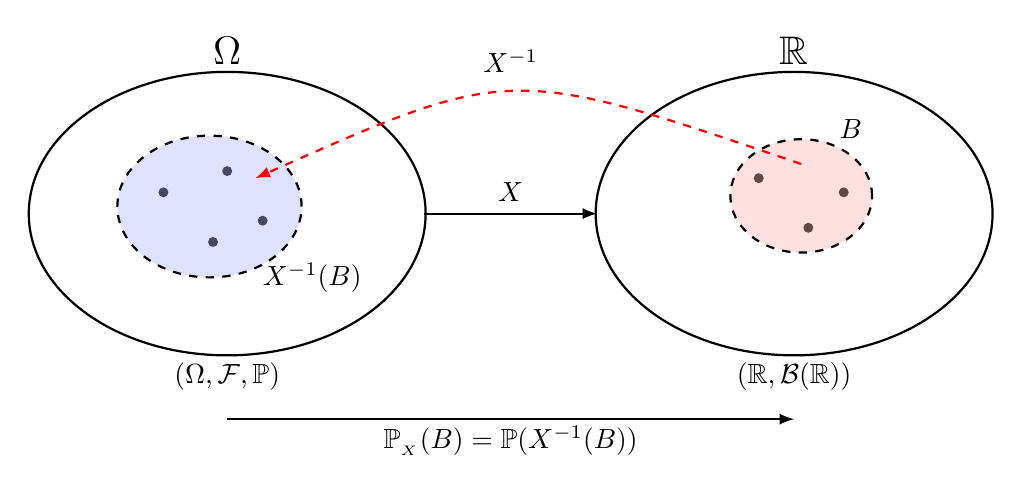
\begin{tikzpicture}[scale=0.9, >=latex]

% --- Sample space Omega ---
\draw[thick] (-4,0) ellipse (2.8 and 2.0);
\node at (-4,2.3) {\Large $\Omega$};
\node at (-4,-2.3) {$(\Omega,\mathcal F,\mathbb P)$};

% sample points in Omega 
\fill (-4.9,0.3) circle (2pt); % in X^{-1}(B)
\fill (-4,0.6) circle (2pt);
\fill (-4.2,-0.4) circle (2pt); % in X^{-1}(B)
\fill (-3.5,-0.1) circle (2pt);

% --- Subset in Omega: X^{-1}(B) ---
\draw[thick, dashed, fill=blue!30, fill opacity=0.4] (-4.25,0.1) ellipse (1.3 and 1.0);
\node at (-2.8,-0.9) {$X^{-1}(B)$};

% --- Real line / codomain ---
\draw[thick] (4,0) ellipse (2.8 and 2.0);
\node at (4,2.3) {\Large $\mathbb R$};
\node at (4,-2.3) {$(\mathbb R,\mathcal B(\mathbb R))$};

% image points in R 
\fill (3.5,0.5) circle (2pt); % in B
\fill (4.2,-0.2) circle (2pt);
\fill (4.7,0.3) circle (2pt); % in B

% --- Subset in R: B  ---
\draw[thick, dashed, fill=red!30, fill opacity=0.4] (4.1,0.25) ellipse (1.0 and 0.8);
\node at (4.8,1.2) {$B$};

% --- Arrow X (stays between the sets) ---
\draw[->, thick] (-1.22,0) -- (1.22,0);
\node at (0,0.3) {$X$};

% --- Dashed inverse image arrow ---
\draw[dashed, thick, red, ->] (4.1,0.7) .. controls (0,2.1) .. (-3.6,0.5);
\node at (0,2.15) {$X^{-1}$};

% --- Probability arrows ---
\draw[->, thick] (-4,-2.9) -- (4,-2.9);
\node at (0,-3.2) {$\mathbb P_{_X}(B)=\mathbb P(X^{-1}(B))$};

		\end{tikzpicture}
\caption{Probability Law For a Random Variable $X$.}
\label{fig:problaw}
	\end{center}
\end{figure}
\vskip 5mm

%%%%%%%%%%%%%%%%%%%%%%%%%%%%%%%%%%%%%%%%%%%%%%%%%%%%%%%%%%%%%%%%%%%%%%%%%%%%%%%%%%%%%%%%%%


A function called the distribution function of $X$ is one of the most important tools for working with random variables.
\vskip 5mm
\begin{defn}
Let $X$ be a random variable with a corresponding probability space $(\O,\F,\P)$. Then we define the {\bf\emph{distribution function}} $F_{_X}$ as
\[F_{_X}(x)=\P_{_X}\Big((-\infty,x]\Big)=\P\Big(\big\{\o\in\O:X(\o)\le x\big\}\Big).\]
\end{defn}

\ni {\bf\emph{Note}}: It can be shown that the distribution function $F_{X}$ completely determines the probability law $\P_{X}$; i.e., once we have defined the probability law for all sets $(-\infty,x]$, there is a unique way to extend this probability law to the Borel $\sigma$-algebra $\mathcal{B}(\R)$.\\

\ni There are a few distinguishing characteristics of a distribution which we list below.\\

\begin{thm}\label{thm:distribution}
Let $(\O,\F,\P)$ be a probability space and $X:\F\to\
R$ be a random variable with distribution function $F_{_X}$. Then the following properties hold.

	\begin{enumerate}
	
		\item $\ds\lim_{x\to-\infty}F_{_X}(x)=0$;
		\item $\ds\lim_{x\to\infty}F_{_X}(x)=1$;
		\item $F_{_X}$ is monotonically increasing everywhere; i.e., if $x\le y$, then $F_{_X}(x)\le F_{_X}(y)$.
		\item $F_{_X}$ is right-continuous; i.e., for all $x\in\R$ we have 
$\ds\lim_{\epsilon\to 0^+}F_{_X}(x+\epsilon)=F_{_X}(x)$. 
		
	\end{enumerate}
	
\end{thm}

\ni There are a limited number of types of random variables: discrete, continuous, singular, or a combination of the previous. In these notes we will only concern ourselves with the definitions of a continuous random variable.


%%%%%%%%%%%%%%%%%%%%%%%%%%%%%%%%%%%%%%%%%%%%%%%%%%%%%%%%%%%%%%%%%%%%%%%%%%%%%%%%%%%%%%%%%%%%%%%%%%%%%%
\section*{Continuous Random Variables:}
%%%%%%%%%%%%%%%%%%%%%%%%%%%%%%%%%%%%%%%%%%%%%%%%%%%%%%%%%%%%%%%%%%%%%%%%%%%%%%%%%%%%%%%%%%%%%%%%%%%%%%


\begin{defn}\label{def:continuous}
A random variable $X$ is called {\bf\emph{continuous}} if for every real number $x \in \mathbb{R}$,
\[\P(X = x) = 0.\]
%Equivalently, the probability that $X$ lies in any interval $[a,b]$ is determined entirely by the cumulative distribution function $F_X$ via
%\[\P(a \le X \le b) = F_X(b) - F_X(a),\]
%and no single point has positive probability.
\end{defn}
\vskip 5mm
We are only interested in the most common type of continuous random variable, called an absolutely continuous random variable.\\

\begin{defn}\label{def:absolute_continuous}
A random variable $X$ is called {\bf\emph{absolutely continuous}} if there exists a non-negative, integrable function $f_{_X}:\mathbb{R} \to [0,\infty)$, called the \emph{probability density function (pdf)}, such that for every Borel set $A \subseteq \mathbb{R}$,
\[\mathbb{P}(X \in A) = \int_A f_{_X}(x)\, dx.\]
Equivalently, the distribution function $F_{_X}$ of $X$ is continuous and can be written as
\[F_{_X}(x) = \mathbb{P}(X \le x) = \int_{-\infty}^{x} f_{_X}(t)\, dt \quad \text{for all } x \in \mathbb{R}.\]
\end{defn}

\ni Some of the most important random variables encountered in probability modeling and statistical theory, such as the uniform distribution or the normal distribution, are continuous random variables. \\


\begin{figure}[h!]
	\begin{center}
		\includegraphics[scale=0.6]{continuous_distribution_plot.jpeg}
\caption{Distribution Function for a Continuous Random Variable.}
\label{fig:crvdistribution}
	\end{center}
\end{figure}	

$\bullet$ The distribution function $F_{_X}$ is continuous everywhere (see Figure~\ref{fig:crvdistribution}), as opposed to the step-type distribution function for a discrete random variable. But we will see with coming examples that it need not be smooth (or differentiable) everywhere.
\vskip 5mm

\ni \emph{Question:} Does the density function represent a probability? That is, do we have $f_{_X}(x)=\P(X=x)$?
\vskip 5mm
The answer is clearly no, because $\P(X=x)=0$ for all $x\in\R$. So how do we interpret the density function of a continuous random variable $X$?


%%%%%%%%%%%%%%%%%%%%%%%%%%%%%%%%%%%%%%%%%%%%%%%%%%%%%%%%%%%%%%%%%%%%%%%%%%%%%%%%%%%%%%%%%%%%%%%%%%%%%%
\section*{Interpreting the Density Function:}
%%%%%%%%%%%%%%%%%%%%%%%%%%%%%%%%%%%%%%%%%%%%%%%%%%%%%%%%%%%%%%%%%%%%%%%%%%%%%%%%%%%%%%%%%%%%%%%%%%%%%%

For a continuous random variable $X$ with density function $f_{_X}$, the value $f_{_X}(x)$ itself is \emph{not} a probability. Instead, the density function should be interpreted as describing how probability is distributed locally along the real line. To make this precise, consider a small positive number $\delta>0$. Then
\[\P(x<X\le x+\delta)=\int_x^{x+\delta} f_{_X}(t)\,dt.\]

If $\delta$ is ``small" and the density function is reasonably smooth near $x$, then $f_{_X}(t)$ does not vary much on the interval $[x,x+\delta]$. In that case, we may approximate the integral by treating the density as approximately constant:
\[\int_x^{x+\delta} f_{_X}(t)\,dt\;\approx\;f_{_X}(x)\,\delta.\]

\ni Thus,
\[\boxed{f_{_X}(x)\,\delta \;\approx\; \mathbb P(x<X\le x+\delta)}\qquad \text{for small } \delta.\]

\medskip

\ni This approximation explains the correct interpretation of a density:
\begin{itemize}
\item $f_{_X}(x)$ measures how \emph{rapidly probability accumulates} near $x$;
\item probabilities arise only after multiplying by a length ($\delta$);
\item smaller intervals lead to better approximations.
\end{itemize}

\ni In geometric terms, $\mathbb P(x<X\le x+\delta)$ is the \emph{area under the density curve} between $x$ and $x+\delta$, while $f_{_X}(x)\delta$ is the area of a rectangle of width $\delta$ and height $f_{_X}(x)$. When $\delta$ is small, these two areas are nearly equal. See Figure~\ref{fig:densityinterpretation}.

\vfill\eject

%%%%%%%%%%%%%%%%%%%%%%%%%%%%%%%%%%%%%%%%%%%%%%%%%%%%%%%%%%%%%%%%%
% Denisty interpretation diagram
%%%%%%%%%%%%%%%%%%%%%%%%%%%%%%%%%%%%%%%%%%%%%%%%%%%%%%%%%%%%%%%%%

\begin{figure}[h!]
\begin{center}
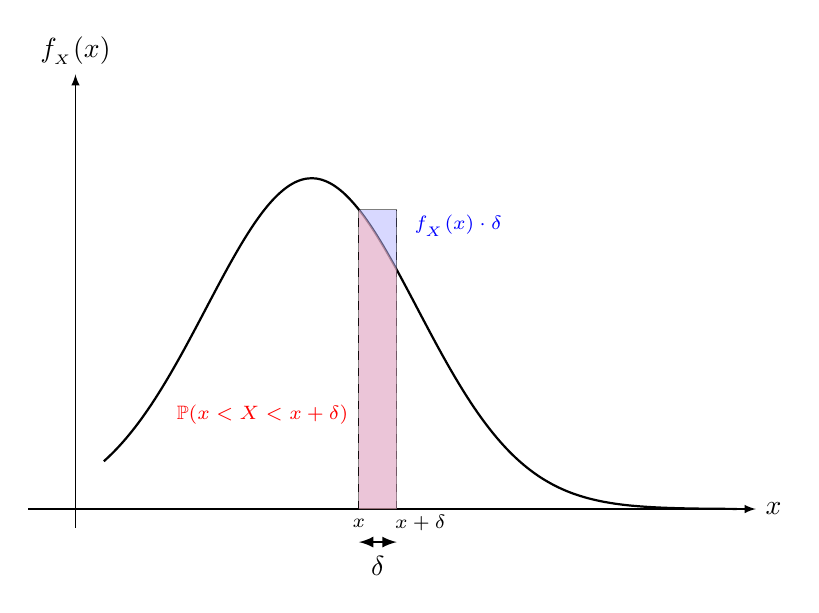
\begin{tikzpicture}[scale=1.2,>=latex]

% Axes
\draw[->] (-0.5,0) -- (7.2,0) node[right] {$x$};
\draw[->] (0,-0.2) -- (0,4.6) node[above] {$f_{_X}(x)$};

% Density curve (scaled up)
\draw[thick, smooth, domain=0.3:7, samples=120]
plot (\x, {3.5*exp(-0.4*(\x-2.5)^2)});

% Interval parameters
\def\xval{3}
\def\deltaval{0.4}

% Vertical dashed lines
\draw[dashed] (\xval,0) -- (\xval,{3.5*exp(-0.4*(\xval-2.5)^2)});
\draw[dashed] (\xval+\deltaval,0) -- (\xval+\deltaval,{3.5*exp(-0.4*(\xval-2.5)^2)});

% Rectangle approximation
\draw[fill=blue!30, opacity=0.5]
(\xval,0) rectangle
(\xval+\deltaval,{3.5*exp(-0.4*(\xval-2.5)^2)});

\node[blue] at (\xval+1.05,3) {\scriptsize $f_{_X}(x)\cdot\delta$};

% Area under curve
\fill[red!30, opacity=0.5]
plot[domain=\xval:\xval+\deltaval, smooth]
(\x,{3.5*exp(-0.4*(\x-2.5)^2)})
-- (\xval+\deltaval,0) -- (\xval,0) -- cycle;

\node[red] at (\xval-1.02,1) {\scriptsize $\P(x<X<x+\delta)$};

% Delta arrow under rectangle
\draw[<->, thick]
(\xval,-0.35) -- (\xval+\deltaval,-0.35);
\node at (\xval,-0.15) {\scriptsize $x$};
\node at (\xval+\deltaval+0.25,-0.15) {\scriptsize $x+\delta$};
\node at (\xval+0.5*\deltaval,-0.6) {$\delta$};

\end{tikzpicture}
\caption{For ``small" $\delta$, the probability $\P(x<X<x+\delta)$ (area under the curve) is well-approximated by the rectangle area $f_{_X}(x)\cdot\delta$.}
\label{fig:densityinterpretation}
\end{center}
\end{figure}




\vskip 1cm
\hrule
\vskip 1cm

%%%%%%%%%%%%%%%%%%%%%%%%%%%%%%%%%%%%%%%%%%%%%%%%%%%%%%%%%%%%%%%%%%%%%%%%%%%%%%%%%%%%%%%%%%%%%%%%%%%%%%
\section*{Theoretical Tools:}
%%%%%%%%%%%%%%%%%%%%%%%%%%%%%%%%%%%%%%%%%%%%%%%%%%%%%%%%%%%%%%%%%%%%%%%%%%%%%%%%%%%%%%%%%%%%%%%%%%%%%%

\noindent Once a continuous random variable is described by its probability density function, we can compute numerical summaries that describe its typical behavior and variability.

\medskip

\begin{defn}
Let $X$ be a continuous random variable with pdf $f_{_X}(x)$.  

\begin{itemize}
\item The \textbf{expected value} (or mean) of $X$ is one measure of the ``center" of the probability distribution. It is computed as 
\[\mathbb{E}[X]=\ds\int^{\infty}_{-\infty}x\,f_{_X}(x)\,dx,\]
provided the integral converges absolutely. It is simply a weighted average.

\item The \textbf{variance} of $X$ is 
\[\mathrm{Var}(X)=\mathbb{E}\big[(X-\mathbb E[X])^2\big]=\ds\int^{\infty}_{-\infty}(x-\mathbb{E}[X])^2 f_{_X}(x)\,dx.\]
This numerical value is a measure of the average squared-distance from the mean which is the center mass of the probability distribution.The variance measures the spread of the distribution around its mean. A commonly used identity is
\[\mathrm{Var}(X)=\mathbb{E}[X^2]-(\mathbb{E}[X])^2.\]
\end{itemize}
\end{defn}

\medskip

\begin{thm*}[Linearity of Expectation]
If $X$ and $Y$ are discrete random variables and $a,b\in\mathbb{R}$, then
\[\mathbb{E}[aX+bY] = a\,\mathbb{E}[X]+b\,\mathbb{E}[Y].\]
This holds \emph{regardless of whether $X$ and $Y$ are independent}.
\end{thm*}

\vskip 2mm

\ni $\bullet$ This property makes expected value one of the most powerful tools in probability.

\vskip 5mm

\begin{thm*}
If $X$ and $Y$ are independent discrete random variables, then
\[\mathrm{Var}(X+Y)=\mathrm{Var}(X)+\mathrm{Var}(Y).\]
\end{thm*}

\medskip

\begin{thm*}[LOTUS]
If $g:\mathbb R\to\R$ is any function, then $Y=g(X)$ is also a discrete random variable with
\[\mathbb{E}[g(X)]=\ds\int^{\infty}_{-\infty}g(x)\,f_{_X}(x)\,dx.\]
\end{thm*}
This theorem is often referred to as the ``law of the unconscious statistician." Notice that to find the expected value of the random variable $g(X)$, we can use the density function for $X$. Conveniently, we do not need to find the density function for the new ranodm variable $g(X)$. This fact is frequently used to compute moments and transformations of random variables.


%%%%%%%%%%%%%%%%%%%%%%%%%%%%%%%%%%%%%%%%%%%%%%%%%%%%%%%%%%%%%%%%%%%%%%%%%%%%%%%%%%%%%%%%%%%%%%%%%%%%%%
\section*{Some Common Continuous Distributions:}
%%%%%%%%%%%%%%%%%%%%%%%%%%%%%%%%%%%%%%%%%%%%%%%%%%%%%%%%%%%%%%%%%%%%%%%%%%%%%%%%%%%%%%%%%%%%%%%%%%%%%%

Many continuous random variables used in modeling arise repeatedly across applications. We briefly introduce several of the most important families, emphasizing their probability density functions, distribution functions, and interpretations.

\subsection*{Uniform Distribution:}

\begin{defn}
A random variable $X$ is said to have a \emph{uniform distribution} on an interval $[a,b]$, written
\[X \sim \mathrm{Uni}(a,b),\]
if its probability density function is
\[f_{_X}(x)=\left\{\begin{array}{ccl}
\ds\frac{1}{b-a}&:& a \le x \le b,\\
\\
0&:&\text{otherwise}.
\end{array}
\right.\]
\end{defn}

\ni The uniform distribution models complete lack of preference: all subintervals of equal length have equal probability. The distribution function is
\[F_{_X}(x)=\left\{\begin{array}{ccl}
0&:&x<a,\\
\ds\frac{x-a}{b-a}&:&a\le x\le b,\\
1&:&x>b.
\end{array}
\right.\]

\ni The expected value and variance are
\[\mathbb{E}[X]=\frac{a+b}{2}, \qquad \mathrm{Var}(X)=\frac{(b-a)^2}{12}.\]

\subsection*{Exponential Distribution:}

\begin{defn}
A random variable $X$ has an \emph{exponential distribution} with rate $\lambda>0$, written
\[X\sim\mathrm{Exp}(\lambda),\]
if its density function is
\[f_{_X}(x)=\left\{\begin{array}{ccl}
\lambda e^{-\lambda x}&:&x\ge 0,\\
0&:&\text{otherwise}.\\
\end{array}
\right.\]
\end{defn}

\ni The distribution function is
\[F_{_X}(x)=1-e^{-\lambda x}, \qquad x\ge 0.\]

\ni The exponential distribution is commonly used to model waiting times until an event occurs (e.g. failure times, arrival times). Its mean and variance are
\[\mathbb E[X]=\frac{1}{\lambda}, \qquad \mathrm{Var}(X)=\frac{1}{\lambda^2}.\]

\ni A key feature is the \emph{memoryless property}:
\[\P(X>s+t \mid X>s)=\mathbb P(X>t).\]

\subsection*{Normal (Gaussian) Distribution:}

\begin{defn}
A random variable $X$ has a \emph{normal distribution} with mean $\mu$ and variance $\sigma^2>0$, written
\[X\sim N(\mu,\sigma^2),\]
if its density function is
\[f_{_X}(x)=\frac{1}{\sqrt{2\pi\sigma^2}}\exp\!\left(-\frac{(x-\mu)^2}{2\sigma^2}\right)\text{ for all } x\in\R.\]
\end{defn}

\ni The expected value and variance are
\[\mathbb{E}[X]=\mu, \qquad \mathrm{Var}(X)=\sigma^2.\]

\ni The normal distribution is symmetric about $\mu$, with $\mu$ representing the center of mass and $\sigma$ controlling the spread. While its distribution function has no closed-form expression, probabilities are well-tabulated and easily computed numerically. Normal distributions arise naturally through aggregation and averaging, a fact formalized by the Central Limit Theorem.

\subsection*{Beta Distribution:}

\begin{defn}
A random variable $X$ has a \emph{beta distribution} with parameters $\alpha>0$ and $\beta>0$, written
\[X\sim\mathrm{Beta}(\alpha,\beta),\]
if its density function is
\[f_{_X}(x)=\left\{\begin{array}{ccl}
\dfrac{1}{B(\alpha,\beta)}\,x^{\alpha-1}(1-x)^{\beta-1}&:& 0\le x\le 1,\\
0&:& \text{otherwise},
\end{array}
\right.\]
where $B(\alpha,\beta)$ is the beta function.
\end{defn}

\ni The beta distribution is flexible and commonly used to model random proportions or probabilities. By adjusting $\alpha$ and $\beta$, the distribution can be symmetric, skewed left or right, or concentrated near the endpoints. See Figure~\ref{fig:betadistribution1}. The mean and variance are
\[\mathbb{E}[X]=\frac{\alpha}{\alpha+\beta},\qquad\mathrm{Var}(X)=\frac{\alpha\beta}{(\alpha+\beta)^2(\alpha+\beta+1)}.\]

\begin{figure}[h!]
	\begin{center}
		\includegraphics[scale=0.7]{beta_distribution_plots1.jpeg}
\caption{Various Densities for $\mathrm{Beta}(\alpha,\beta)$ random variables.}
\label{fig:betadistribution1}
	\end{center}
\end{figure}	

%%%%%%%%%%%%%%%%%%%%%%%%%%%%%%%%%%%%%%%%%%%%%%%%%%%%%%%%%%%%%%%%%%%%%%%%%%%%%%%%%%%%%%%%%%%%%%%%%%%%%%
\section*{Foundational Examples:}
%%%%%%%%%%%%%%%%%%%%%%%%%%%%%%%%%%%%%%%%%%%%%%%%%%%%%%%%%%%%%%%%%%%%%%%%%%%%%%%%%%%%%%%%%%%%%%%%%%%%%%

The following examples highlight how probability density functions are used to compute probabilities and expectations.

\subsection*{Example 1: Probability as Area}

Let $X\sim\mathrm{Uni}(0,4)$. Compute $\mathbb P(1\le X\le 3)$. Since the density is constant on $[0,4]$,
\[\P(1\le X\le 3)=\int_1^3 \frac{1}{4}\,dx=\frac{1}{2}.\]

\ni This emphasizes the geometric interpretation of probability as area under the density curve.

\subsection*{Example 2: Point Probabilities}

Let $X\sim\mathrm{Exp}(2)$. Compute $\mathbb P(X=1)$. Since $X$ is continuous,
\[\P(X=1)=\int_1^1 2e^{-2x}\,dx=0.\]

\ni This reinforces the idea that density values are not probabilities, but rather \emph{rates} at which probability accumulates.

\subsection*{Example 3: Using the Distribution Function}

Let $X\sim N(0,1)$. Express $\mathbb P(|X|\le 1)$ using the distribution function. By symmetry,
\[\P(|X|\le 1)=F_{_X}(1)-F_{_X}(-1).\]

\ni Numerical values are obtained using tables or software.

\subsection*{Example 4: Expected Value from a Density}

Suppose $X$ has density
\[f_{_X}(x)=\left\{\begin{array}{ccl}
2x&:&0\le x\le 1,\\
0&:&\text{otherwise}.
\end{array}
\right.\]

\ni Then
\[\mathbb{E}[X]=\int_0^1 x(2x)\,dx=\frac{2}{3}.\]

\ni This example illustrates expectation as a weighted average of all possible values.

\subsection*{Example 5: Interpreting Shape}

Using Figure~\ref{fig:betadistribution2}, compare the densities of $\mathrm{Beta}(5,2)$, $\mathrm{Beta}(30,30)$, and $\mathrm{Beta}(0.5,0.5)$. Although all are supported on $[0,1]$, their shapes differ dramatically, illustrating how parameters influence modeling assumptions about concentration and variability.

\begin{figure}[h!]
	\begin{center}
		\includegraphics[scale=0.7]{beta_distribution_plots2.jpeg}
\caption{Various Densities for $\mathrm{Beta}(\alpha,\beta)$ random variables.}
\label{fig:betadistribution2}
	\end{center}
\end{figure}	

\vskip 1cm
\hrule
\vskip 1cm


%%%%%%%%%%%%%%%%%%%%%%%%%%%%%%%%%%%%%%%%%%%%%%%%%%%%%%%%%%%%%%%%%%%%%%%%%%%%%%%%%%%%%%%%%%%%%%%%%%%%%%
\section*{Practice Problems: Common Continuous Distributions}
%%%%%%%%%%%%%%%%%%%%%%%%%%%%%%%%%%%%%%%%%%%%%%%%%%%%%%%%%%%%%%%%%%%%%%%%%%%%%%%%%%%%%%%%%%%%%%%%%%%%%%

The following exercises are designed to reinforce the interpretation and use of common continuous random variables. Unless otherwise stated, all random variables are assumed to be absolutely continuous.

\subsection*{Uniform Distribution}

\begin{enumerate}
\item Let $X\sim\mathrm{Uni}(2,6)$.
\begin{enumerate}
    \item Write down the probability density function $f_{_X}(x)$.
    \item Compute $\mathbb P(3\le X\le 5)$.
    \item Compute $\mathbb P(X>4)$.
    \item Find $\mathbb E[X]$ and $\mathrm{Var}(X)$.
\end{enumerate}

\item Suppose $X\sim\mathrm{Uni}(0,1)$.
\begin{enumerate}
    \item Compute $\mathbb P(X=0.5)$.
    \item Explain why this result does not contradict the fact that $f_{_X}(0.5)=1$.
\end{enumerate}
\end{enumerate}

\subsection*{Exponential Distribution}

\begin{enumerate}
\item Let $X\sim\mathrm{Exp}(3)$.
\begin{enumerate}
    \item Compute $\mathbb P(X>1)$.
    \item Compute $\mathbb P(1<X<2)$.
    \item Find $\mathbb E[X]$.
\end{enumerate}

\item Suppose $X\sim\mathrm{Exp}(\lambda)$ represents the waiting time (in hours) until a system fails.
\begin{enumerate}
    \item Interpret $\mathbb P(X>5)$ in words.
    \item Show that $\mathbb P(X>s+t\mid X>s)=\mathbb P(X>t)$.
    \item Explain, in words, why this property is called \emph{memoryless}.
\end{enumerate}
\end{enumerate}

\subsection*{Normal Distribution}

\begin{enumerate}
\item Let $X\sim N(10,4)$.
\begin{enumerate}
    \item State the mean and standard deviation of $X$.
    \item Express $\mathbb P(8<X<12)$ using the distribution function $F_{_X}$.
\end{enumerate}

\item Suppose $X\sim N(0,1)$.
\begin{enumerate}
    \item Express $\mathbb P(|X|>2)$ in terms of $F_{_X}$.
    \item Explain why symmetry of the normal distribution simplifies this computation.
\end{enumerate}
\end{enumerate}

\subsection*{Beta Distribution}

\begin{enumerate}
\item Let $X\sim\mathrm{Beta}(2,5)$.
\begin{enumerate}
    \item On which interval is $X$ supported?
    \item Is the distribution skewed left or right? Justify your answer.
    \item Compute $\mathbb E[X]$.
\end{enumerate}

\item Consider the following beta distributions: $\mathrm{Beta}(1,1)$, $\mathrm{Beta}(30,30)$, and $\mathrm{Beta}(0.5,0.5)$.
\begin{enumerate}
    \item Which corresponds to a uniform distribution?
    \item Which places more probability near $0$ and $1$?
    \item Which best represents prior belief that a probability is near $0.5$?
\end{enumerate}
\end{enumerate}

\subsection*{Conceptual and Mixed Problems}

\begin{enumerate}
\item Let $X$ be a continuous random variable with density $f_{_X}$.
\begin{enumerate}
    \item Explain why $f_{_X}(x)\,\delta$ is an approximation to $\mathbb P(x<X<x+\delta)$ for small $\delta$.
    \item Describe how this approximation improves as $\delta\to 0$.
\end{enumerate}

\item Suppose two continuous random variables have the same distribution function.
\begin{enumerate}
    \item What can you say about their probability laws?
    \item Must they be defined on the same sample space?
\end{enumerate}

\item A student claims:  
\emph{“Since the density function is large near $x=2$, the probability that $X=2$ must also be large.”}
\begin{enumerate}
    \item Explain why this statement is incorrect.
    \item Rewrite the statement so that it is correct.
\end{enumerate}
\end{enumerate}


%\vskip 1cm
%\hrule
%\vskip 1cm

\vfill\eject

%%%%%%%%%%%%%%%%%%%%%%%%%%%%%%%%%%%%%%%%%%%%%%%%%%%%%%%%%%%%%%%%%%%%%%%%%%%%%%%%%%%%%%%%%%%%%%%%%%%%%%
\section*{Solutions to Practice Problems:}
%%%%%%%%%%%%%%%%%%%%%%%%%%%%%%%%%%%%%%%%%%%%%%%%%%%%%%%%%%%%%%%%%%%%%%%%%%%%%%%%%%%%%%%%%%%%%%%%%%%%%%

\subsection*{Uniform Distribution}

\begin{solutionbox}
\textbf{Problem 1.} Let $X\sim\mathrm{Unif}(2,6)$.

\begin{enumerate}
\item The density is
\[f_{_X}(x)=\left\{\begin{array}{ccl}
\dfrac{1}{4}&:& 2\le x\le 6,\\
\\
0&:& \text{otherwise}.
\end{array}
\right.\]

\item
\[\mathbb P(3\le X\le 5)=\int_3^5 \frac{1}{4}\,dx=\frac{2}{4}=\frac{1}{2}.\]

\item
\[\P(X>4)=\int_4^6 \frac{1}{4}\,dx=\frac{2}{4}=\frac{1}{2}.\]

\item
\[\mathbb{E}[X]=\frac{2+6}{2}=4,\qquad\mathrm{Var}(X)=\frac{(6-2)^2}{12}=\frac{4}{3}.\]
\end{enumerate}
\end{solutionbox}

%%%%%%%%%%%%%%%%%%
\vskip 1cm
%%%%%%%%%%%%%%%%%%

\begin{solutionbox}
\textbf{Problem 2.} Let $X\sim\mathrm{Uni}(0,1)$.

\begin{enumerate}
\item
\[\P(X=0.5)=0,\]
since $X$ is continuous.

\item This does not contradict $f_{_X}(0.5)=1$ because the density function is \emph{not} a probability. Probabilities are obtained by integrating the density over intervals, not by evaluating it at a point.
\end{enumerate}
\end{solutionbox}

%%%%%%%%%%%%%%%%%%%%%%%%%%%%%%%%%%%%%%%%%%%%%%%%%%%%%%%%%%%%%%%%%%%%%%%

\subsection*{Exponential Distribution}

\begin{solutionbox}
\textbf{Problem 3.} Let $X\sim\mathrm{Exp}(3)$.

\begin{enumerate}
\item
\[\P(X>1)=e^{-3}.\]

\item
\[\P(1<X<2)=\ds\int_1^2 3e^{-3x}\,dx=e^{-3}-e^{-6}.\]

\item
\[\mathbb{E}[X]=\frac{1}{3}.\]
\end{enumerate}
\end{solutionbox}


%%%%%%%%%%%%%%%%%%
\vskip 1cm
%%%%%%%%%%%%%%%%%%


\begin{solutionbox}
\textbf{Problem 4.}

\begin{enumerate}
\item $\P(X>5)$ is the probability that the system lasts more than 5 hours without failing.

\item
\[\P(X>s+t\mid X>s)=\frac{\mathbb P(X>s+t)}{\P(X>s)}=\frac{e^{-\lambda(s+t)}}{e^{-\lambda s}}=e^{-\lambda t}.\]

\item The conditional distribution does not depend on how long the system has already survived, which is why the distribution is called \emph{memoryless}.
\end{enumerate}
\end{solutionbox}

%%%%%%%%%%%%%%%%%%%%%%%%%%%%%%%%%%%%%%%%%%%%%%%%%%%%%%%%%%%%%%%%%%%%%%%

\subsection*{Normal Distribution}

\begin{solutionbox}
\textbf{Problem 5.} Let $X\sim N(10,4)$.

\begin{enumerate}
\item Mean $=10$, standard deviation $=2$.

\item
\[\P(8<X<12)=F_{_X}(12)-F_{_X}(8).\]
\end{enumerate}
\end{solutionbox}


%%%%%%%%%%%%%%%%%%
\vskip 1cm
%%%%%%%%%%%%%%%%%%


\begin{solutionbox}
\textbf{Problem 6.} Let $X\sim N(0,1)$.

\begin{enumerate}
\item
\[\P(|X|>2)=1-\big(F_{_X}(2)-F_{_X}(-2)\big).\]

\item By symmetry,
\[\P(|X|>2)=2\,\mathbb P(X>2).\]
\end{enumerate}
\end{solutionbox}

%%%%%%%%%%%%%%%%%%%%%%%%%%%%%%%%%%%%%%%%%%%%%%%%%%%%%%%%%%%%%%%%%%%%%%%

\subsection*{Beta Distribution}

\begin{solutionbox}
\textbf{Problem 7.} Let $X\sim\mathrm{Beta}(2,5)$.

\begin{enumerate}
\item The support is $[0,1]$.

\item Since $\beta>\alpha$, the distribution is skewed toward $0$ (right-skewed).

\item
\[\mathbb{E}[X]=\frac{2}{2+5}=\frac{2}{7}.\]
\end{enumerate}
\end{solutionbox}


%%%%%%%%%%%%%%%%%%
\vskip 1cm
%%%%%%%%%%%%%%%%%%

\begin{solutionbox}
\textbf{Problem 8.}

\begin{enumerate}
\item $\mathrm{Beta}(1,1)$ is uniform on $[0,1]$.

\item $\mathrm{Beta}(0.5,0.5)$ places more probability near $0$ and $1$.

\item $\mathrm{Beta}(2,2)$ best represents belief concentrated near $0.5$.
\end{enumerate}
\end{solutionbox}

%%%%%%%%%%%%%%%%%%%%%%%%%%%%%%%%%%%%%%%%%%%%%%%%%%%%%%%%%%%%%%%%%%%%%%%

\subsection*{Conceptual and Mixed Problems}

\begin{solutionbox}
\textbf{Problem 9.}

\begin{enumerate}
\item
\[\P(x<X<x+\delta)=\int_x^{x+\delta} f_{_X}(t)\,dt\approx f_{_X}(x)\,\delta\]
when $\delta$ is small and $f_{_X}$ varies slowly.

\item As $\delta\to 0$, the approximation improves because the density is nearly constant over smaller intervals.
\end{enumerate}
\end{solutionbox}


%%%%%%%%%%%%%%%%%%
\vskip 1cm
%%%%%%%%%%%%%%%%%%


\begin{solutionbox}
\textbf{Problem 10.}

\begin{enumerate}
\item If two random variables have the same distribution function, they have the same probability law.

\item They do \emph{not} need to be defined on the same sample space.
\end{enumerate}
\end{solutionbox}


%%%%%%%%%%%%%%%%%%
\vskip 1cm
%%%%%%%%%%%%%%%%%%


\begin{solutionbox}
\textbf{Problem 11.}

\begin{enumerate}
\item The statement is incorrect because $\mathbb P(X=x)=0$ for continuous random variables.

\item A correct statement is:  
\emph{“A large value of $f_{_X}(x)$ indicates that $X$ is more likely to lie near $x$ than near points where the density is smaller.”}
\end{enumerate}
\end{solutionbox}


%%%%%%%%%%%%%%%%%%%%%%%%%%%%%%%%%%%%%%%%%%%%%%%%%%%%%%%%%%%%%%%%%%%%%%%%%%%%%%%%%%%%%%%%%%%%%%%%%%%%%%%
%\section*{The R Code:} 
%%%%%%%%%%%%%%%%%%%%%%%%%%%%%%%%%%%%%%%%%%%%%%%%%%%%%%%%%%%%%%%%%%%%%%%%%%%%%%%%%%%%%%%%%%%%%%%%%%%%%%%
% Here is the R code used for the above simulations.
%\vspace*{2mm}
%\small 
%\begin{lstlisting}[language=R]
%
%
%
%\end{lstlisting}



\vskip 1cm
\hrule
\vskip 5mm
\begin{center}
\bf Please let me know if you have any questions, comments, or corrections!
\end{center}

%%%%%%%%%%%%%%%%%%%%%%%%%%%%%%%%%%%%%%%%%%%%%%%%%%%%%%
\end{document}
%%%%%%%%%%%%%%%%%%%%%%%%%%%%%%%%%%%%%%%%%%%%%%%%%%%%%%

